\documentclass{article}
\usepackage[margin=1in]{geometry}
\usepackage{amsmath,amsfonts,amssymb}
\usepackage{listings}
\usepackage{color}
\usepackage{graphicx}
\usepackage{subfig}
\usepackage{blkarray}
\usepackage{multirow}
\usepackage{float}
\usepackage{caption}
\usepackage{subcaption}
\begin{document}
\begin{titlepage}
	\setlength{\parindent}{0pt}
	\large

\vspace*{-2cm}

\definecolor{dkgreen}{rgb}{0,0.6,0}
\definecolor{gray}{rgb}{0.5,0.5,0.5}
\definecolor{mauve}{rgb}{0.58,0,0.82}

\lstset{frame=tb,
  language=Python,
  aboveskip=3mm,
  belowskip=3mm,
  showstringspaces=false,
  columns=flexible,
  basicstyle={\small\ttfamily},
  numbers=none,
  numberstyle=\tiny\color{gray},
  keywordstyle=\color{blue},
  commentstyle=\color{dkgreen},
  stringstyle=\color{mauve},
  breaklines=true,
  breakatwhitespace=true,
  tabsize=3
}

University of Waterloo \par
CS 480 \par
\vspace{0.05cm}
r2knowle: 2023-11-28
\vspace{0.2cm}

{\huge Exercise \# 4 \par}
\hrule

\vspace{0.5cm}
\textbf{Q4a)} Below we can see the accuracy of the membership inference attack on both the cheating and generalized dataset:

\begin{tabular}{ll}

 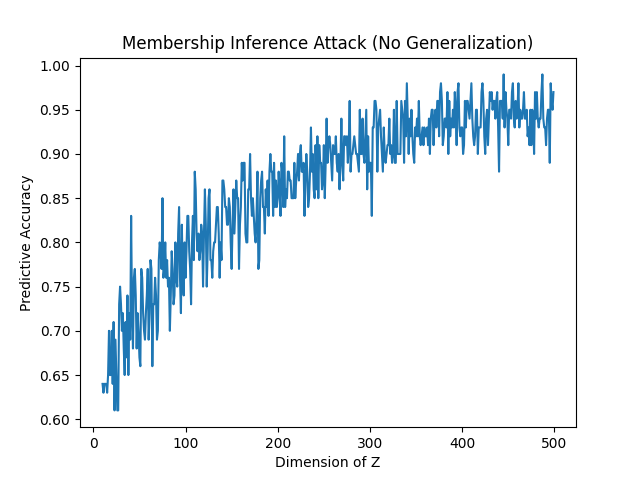
\includegraphics[width=.5\linewidth]{q4a1.png} &  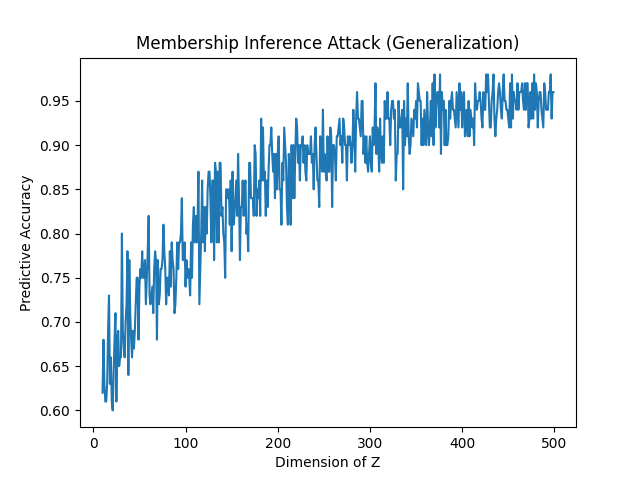
\includegraphics[width=.5\linewidth]{q4a2.png}\\
 \hfil (i) Attacks on "cheating" dataset  \hfil & \hfil (ii) Distribution of unique testing observations \hfil \\\\
 
\end{tabular}

From this we can see that there appears to be an upper bound that both the cheating and generalized dataset run into, we also see that this upper bound is far better then random guessing as there would only be a $50\%$ change of getting it right, but with this attack we can achieve accuracy's of upto $80\%$. \\

For this next part we are going to graph the effectiveness of protecting against each attack, the first graph shows us how $||u||_2$ changes with $\sigma$ which demonstrates how the accuracy of our model will change. We will also show how the effectiveness of this attack changes with different values of $\sigma$:

\begin{tabular}{ll}

 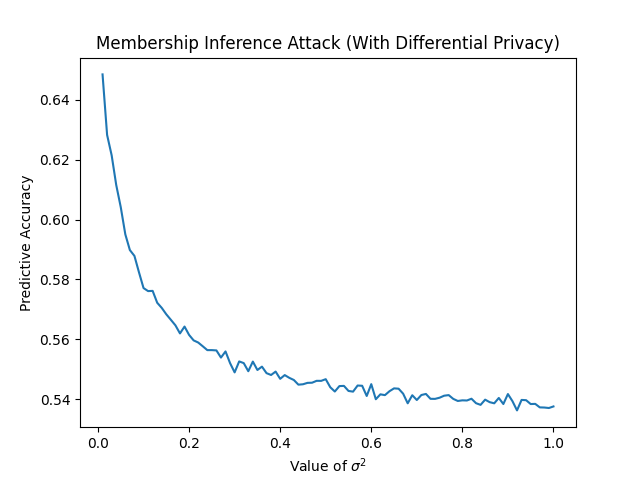
\includegraphics[width=.5\linewidth]{4b.png} &  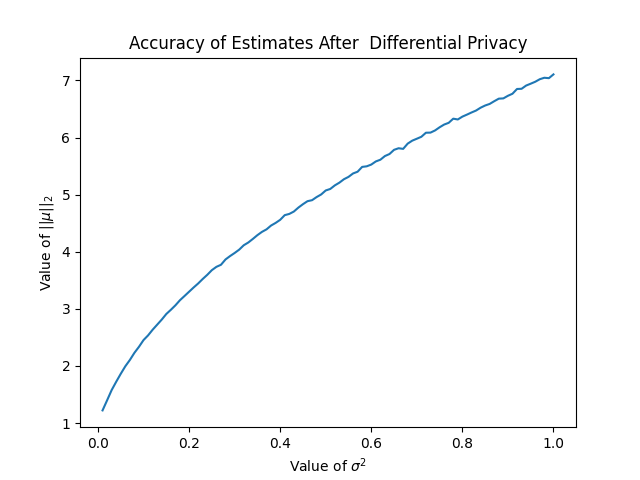
\includegraphics[width=.5\linewidth]{Q4B.png}\\
 \hfil (i) Effectiveness of defences  \hfil & \hfil (ii) Loss in accuracy of estimates \hfil \\\\
 
\end{tabular}
From this we can see that as our model becomes more resistants to attacks, it also becomes less accurate. However since effectiveness of defenses has diminishing returns there is a point that maximizes both.
\newpage
\textbf{Q4b)} Before doing any membership inference attacks, we get the following accuracies on both the test and training set using logistic regression:
\begin{center}
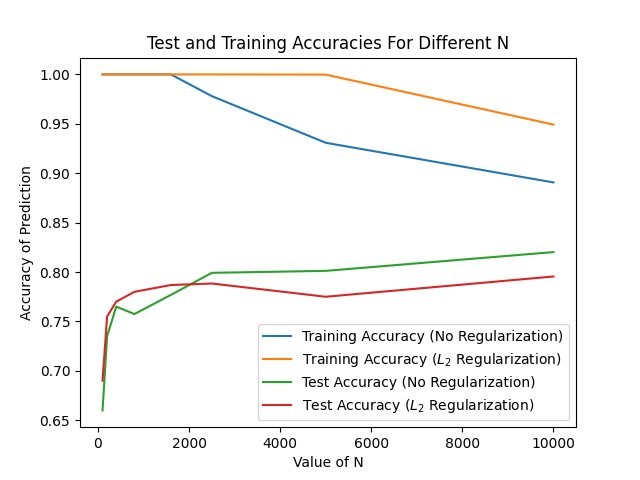
\includegraphics[width=.6\linewidth]{Q4c.png}
\end{center}
On really small N it makes sense that the training accuracy would be perfect, as each sample would be unique and so the boundary between each prediction would be large. Therefore as N gets larger it makes sense that the training accuracy would drop, it also makes sense that the test accuracy would increase and converge to a point as we are no longer under fitting.
\begin{center}
\includegraphics[width=.6\linewidth]{Q4d.png}
\end{center}
At very small Ns, as seen in the graph above our test accuracy would be very low and our training accuracy very high. This means our estimates for the IN group and OUT group would be very accurate, and so the attack accuracy would be high. As N increases and our model does worse with training and better with test it makes sense that the attack accuracy would also drop.
\newpage
To defend against this attack we will be modifying the parameter vector of our logistic regression model. After doing so we get two graphs, the first shows the effectiveness of defences and the second shows the loss in accuracy of predictions:

\begin{tabular}{ll}

 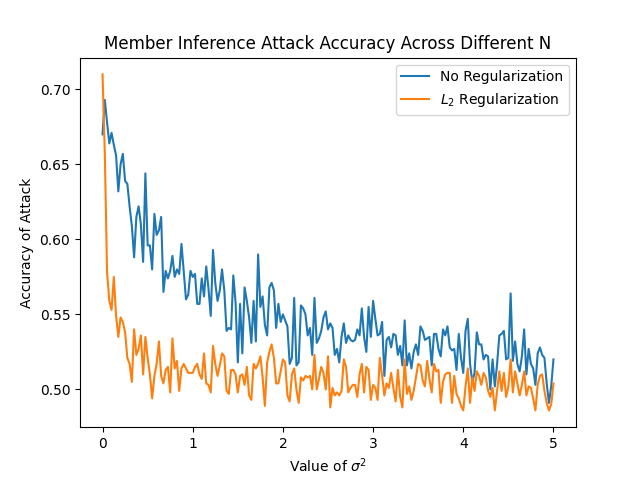
\includegraphics[width=.5\linewidth]{q4f.png} &  \includegraphics[width=.5\linewidth]{Q4g.png}\\
 \hfil (i) Effectiveness of defences  \hfil & \hfil (ii) Loss in accuracy of estimates \hfil \\\\
 
\end{tabular}
We can see that predictive accuracy drops off as sigma increases, and as a result our membership inference attack becomes less and less effective. This simulates what we got from the graphs if Q4a. We notice that l2 regularization is effected more by changes in Gaussian noise then the no regularization term, and that overall because of this it is less impacted by membership inference attacks.
\end{titlepage}
\end{document}